% !TeX spellcheck = pl_PL
\documentclass[a4paper,twoside]{article}
\usepackage{polski}
\usepackage[utf8]{inputenc}
\usepackage{graphicx}
\usepackage{amsmath}

\usepackage[unicode, bookmarks=true]{hyperref} %do zakładek
\usepackage{tabto} % do tabulacji
\NumTabs{6} % globalne ustawienie wielkosci tabulacji
\usepackage{array}
\usepackage{multirow}
\usepackage{array}
\usepackage{dcolumn}
\usepackage{bigstrut}
\usepackage{color}
\usepackage[usenames,dvipsnames]{xcolor}
\usepackage{svg}
\usepackage{xfrac}
\usepackage{floatrow}
\usepackage{enumitem}
\usepackage{listings,lstautogobble}


\usepackage{multirow,tabularx}
\newcolumntype{Y}{>{\centering\arraybackslash}X}
\renewcommand{\arraystretch}{2}

% === Reset inkrementacji sekcji przy nowym parcie === %
\usepackage{titlesec}

\makeatletter
\@addtoreset{section}{part}
\makeatother
\titleformat{\part}[display]
{\normalfont\LARGE\bfseries\centering}{}{-60pt}{}

% === Dodanie krpki do sekcji
\titlelabel{\thetitle.\quad}


\setlength{\textheight}{24cm}
\setlength{\textwidth}{15.92cm}
\setlength{\footskip}{10mm}
\setlength{\oddsidemargin}{0mm}
\setlength{\evensidemargin}{0mm}
\setlength{\topmargin}{0mm}
\setlength{\headsep}{5mm}

\setlength{\textfloatsep}{10pt plus 1.0pt minus 2.0pt}


\begin{document}
	\bibliographystyle{plain}
	
	% ************************************************************
	% --- Strona tytułowa
	% ************************************************************
	\begin{titlepage}
		\begin{table}[htbp]
			\centering
			\begin{tabular}{|c|c|c|c|c|c|c|}
				\hline
				\multicolumn{7}{|c|}{\textbf{{\LARGE Grafika Komputerowa}}} \bigstrut\\[4pt]
				\hline
				Rok akademicki & Termin & Rodzaj studiów & Kierunek & Prowadzący & Grupa & Sekcja \bigstrut\\
				\hline
				\multicolumn{1}{|c|}{\multirow{2}[4]{*}{{\large 2014/2015}}} & \multicolumn{1}{c|}{{\large Piątek}} & \multicolumn{1}{c|}{\multirow{2}[4]{*}{{\large SSI}}} & \multicolumn{1}{c|}{\multirow{2}[4]{*}{{\large INF}}} & \multicolumn{1}{c|}{\multirow{2}[4]{*}{\begin{tabular}{@{}c@{}}{\large dr} \\[-9pt] {\large Ewa Lach}\end{tabular}}} & \multicolumn{1}{c|}{\multirow{2}[4]{*}{{\large GKiO3}}} & \multicolumn{1}{c|}{\multirow{2}[4]{*}{{\large 1}}} \bigstrut\\
				\cline{2-2}    \multicolumn{1}{|c|}{} & \multicolumn{1}{c|}{{\large 09:30 - 11:00}} & \multicolumn{1}{c|}{} & \multicolumn{1}{c|}{} & \multicolumn{1}{c|}{} & \multicolumn{1}{c|}{} & \multicolumn{1}{c|}{} \bigstrut\\
				\hline
			\end{tabular}%
		\end{table}%
		
		\centering
		\includegraphics[width=0.6\textwidth]{./images/logo.png}
		\\\vspace{10mm}
		\textbf{{\huge Karta projektu}}\\\vspace{5mm}
		\textbf{{\Huge Danmaku Shooter}}
		\\
		\vfill
		\begin{flushright}
			{\Large \textbf{Skład sekcji}:}\\
			\begin{tabular}{rr}
				{\Large Buchała} & {\Large Bartłomiej}\\[-3pt]
				{\Large Forczmański} & {\Large Mateusz}\\[-3pt]
				{\Large Motyka} & {\Large Marek}\\[-3pt]
				{\Large Wudecki} & {\Large Wojciech}
			\end{tabular}
		\end{flushright}
		
	\end{titlepage}
	
	
	
	% ************************************************************
	% --- Strona z założeniami
	% ************************************************************
	\part{\huge \textbf{Krótki opis aplikacji}}
	\textit{Shoot' em up} (w skrócie zwany shmup) jest gatunkiem gier akcji wywodzącym się w prostej linii od gier typu \textit{Space Invaders} lub \textit{River Raid}. Kontrolowana przez gracza postać (np. statek) w pojedynkę stawia czoło przeciwnikom, niszcząc ich za pomocą wystrzeliwanych pocisków, jednocześnie unikając ich ataków. Podgatunek shmupów, zwany \textit{danmaku} (z jap. \textit{ściana pocisków} lub \textit{piekło pocisków}) kładzie większy nacisk na omijanie wrogich ataków, niż na ofensywie. Przykładowymi danmaku są np. \textit{Ikaruga} czy większość gier z uniwersum \textit{Touhou Project}. \\
	
	Gra powstawać będzie jako projekt łączony z przedmiotów Projekt Programistyczny i Grafika Komputerowa.
	
	\begin{center}
		\fbox{%
			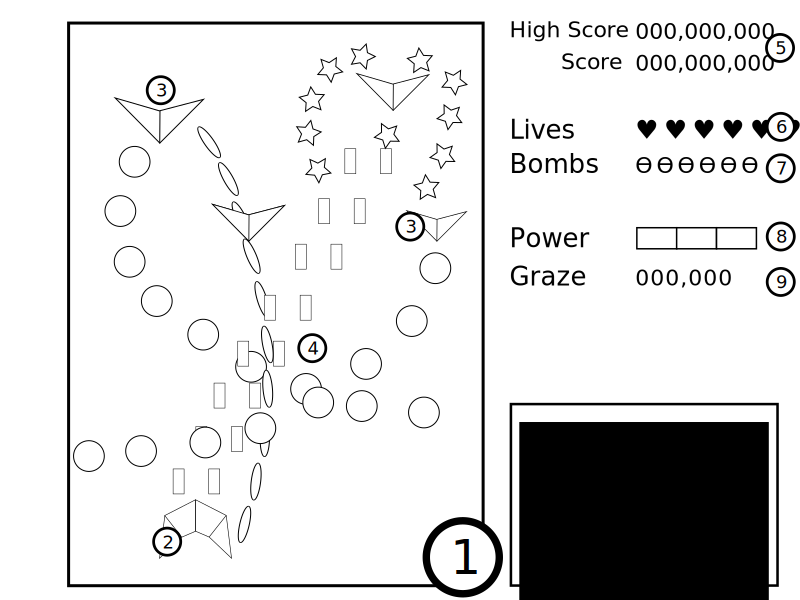
\includegraphics[width=0.8\textwidth]{./images/screen01}%
		}
		\vspace{5pt}
	\end{center}
	\begin{enumerate}
		\item Ekran gry właściwej. W jej obrębie znajduje się gracz, pociski oraz wszyscy wrogowie. 
		\item Grywalna postać, porusza się po ekranie gry, unikając pocisków oraz strzelając do wrogów.
		\item Wrogowie, których należy pokonać.
		\item Chmara pocisków. Jak widać na rysunku, nie wchodzą ze sobą w żadną interakcję, każdy leci swoim wyznaczonym torem. Sprajty wrogów są niewrażliwe na swoje pociski, nie występuje \textit{friendly fire}.
		\item Liczba zdobytych punktów oraz porównywanie ich z największym wynikiem.
		\item Liczba pozostałych żyć. W trakcie gry można zdobywać kolejne. Utrata wszystkich kończy grę.
		\item Liczba pozostałych bomb. Każda wykorzystana bomba zapewnia kilkusekundową odporność na wrogie pociski oraz umożliwia pojedynczy silniejszy atak. Można je zdobyć w trakcie gry.
		\item Pasek mocy, napełnia się w trakcie gry wraz ze zdobytymi punktami. Utrata życia skutkuje zmniejszeniem paska o 1 segment.
		\item Liczba "otarć", czyli uniknięć bardzo blisko pocisku. Aby umożliwić większe wyzwanie, ostateczny wynik pomnożony jest przez licznik Graze.
	\end{enumerate}
	
	
	\newpage
	
	\part{\huge \textbf{Analiza zadania}}
	
	\section{Podstawy teoretyczne problemu}
	\subsection{Przestrzeń fizyczna}
	W naszej grze w interakcję ze sobą będzie wchodzić bardzo dużo elementów, począwszy od gracza, a na ostatnim z setki pocisków skończywszy. Bardzo ważne jest, aby ruchy i interakcje wszystkich elementów były ze sobą zsynchronizowane, a droga o długości 1 była tym samym dla każdego z nich.\\
	W tym celu zdecydowaliśmy się na wprowadzenie do gry przestrzeni fizycznej, w której będą zachodzić wybrane przez nas zjawiska fizyczne, potrzebne dla realizacji gry.
	
	\subsection{Ruch}
	Każdy obiekt, który może się poruszać i zmienić swoje położenia, posiada swoją prędkość. W naszej grze wyróżniliśmy 3 rodzaje ruchu:
	\subsubsection{Ruch jednostajny}
	W jednostce czasu ciało pokonuje jednakową drogę, a przebyta droga jest proporcjonalna do czasu.
	$$ v=\cfrac{s}{t}=const$$
	Gdzie $ v $ to prędkość, $ s $ - droga, a $ t $ to czas. W naszym obiekty poruszają się na ekranie, więc jednostką długości jest piksel.
	\subsubsection{Ruch jednostajnie przyspieszony}
	W jednostce czasu prędkość ciała ulega zwiększeniu o stałą wartość.
	$$ v(t)=v_0+a\cdot t $$
	\subsubsection{Ruch jednostajnie opóźniony}
	W jednostce czasu prędkość ciała ulega pomniejszeniu o stałą wartość.
	$$ v(t)=v_0-a\cdot t $$
	
	\subsection{Tor pocisków}
	Jednym z podstawowych problemów w naszym zadaniu jest tor po jakim poruszają się pociski. Obiekty wrogów będą poruszać się w prosty sposób, jednak zbiory pocisków będą układać się w skomplikowane wzory, tworzyć ze sobą specyficzny układ. W naszej grze chcemy zaimplementować pociski, które będą poruszać się m.in. po takich torach jak okrąg i elipsa.\\
	
	\subsubsection{Okrąg}
	$$
	\begin{cases}
	x=x_0+r\cdot \cos{\theta}\\
	y=y_0+r\cdot \sin{\theta}
	\end{cases}
	$$
	Gdzie punkt $ O(x_0, y_0) $ jest środkiem okręgu, $ r $ promieniem, a parametr $ \theta \in [0, 2\pi ) $.
	\subsubsection{Elipsa}
	Podobnie jak wyżej, elipsę zdefiniowaliśmy równaniem parametrycznym:
	$$
	\begin{cases}
	x=x_0+a\cdot \cos{\theta}\\
	y=y_0+b\cdot \sin{\theta}
	\end{cases}
	$$
	Gdzie punkt $ O(x_0, y_0) $ jest środkiem elipsy, $ a,\:b $ długościami półosi, a parametr $ \theta \in [0, 2\pi ) $.
	\subsubsection{Spirala}
	Będziemy wykorzystywać spirale z gatunku spiral Archimedesa. Tor takiej spirali jest zdefiniowany równaniem parametrycznym:
	$$
	\begin{cases}
	x=x_0+a\cdot \theta \cdot \cos{\theta}\\
	y=y_0+a\cdot \theta \cdot \sin{\theta}
	\end{cases}
	$$
	Gdzie punkt $ O(x_0, y_0) $ jest punktem centralnym spirali, $ a \in R $ , a parametr $ \theta \in [0, \inf ) $.
	\subsubsection{Spirala Fermata}
	Typ spirali zdefiniowany równaniem parametrycznym:
	$$
	\begin{cases}
	x=x_0+a\cdot \sqrt{\theta} \cdot \cos{\theta}\\
	y=y_0+a\cdot \sqrt{\theta} \cdot \sin{\theta}
	\end{cases}
	$$
	Gdzie punkt $ O(x_0, y_0) $ jest punktem centralnym spirali, $ a \in R $, a parametr $ \theta \in [-inf, \inf ) $.
	\subsubsection{Spirala hiperboliczna}
	Typ spirali zdefiniowany równaniem parametrycznym:
	$$
	\begin{cases}
	x=x_0+ae^{b\theta} \cdot \cos{\theta}\\
	y=y_0+ae^{b\theta} \cdot \sin{\theta}
	\end{cases}
	$$
	Gdzie punkt $ O(x_0, y_0) $ jest punktem centralnym spirali, $ a,b \in R $, a parametr $ \theta \in [0, \inf ) $.
	
	\newpage
	\section{Wykorzystywane zagadnienia grafiki komputerowej}
	\subsection{Przekształcenia afiniczne}
	Postanowiliśmy wykorzystać poznane na laboratorium przekształcenia afiniczne. Wszystkie ruchome obiekty w naszej grze, które zmieniają dynamicznie swoją pozycję w przestrzeni dwuwymiarowej, będą korzystać z trzech wybranych przekształceń:
	\subsubsection{Translacja}
	Przesunięcie punktu $ P=(x, y) $ o wektor $ d=[d_x, d_y] $, w wyniku którego powstaje obraz\\ $ P=(x', y') $, gdzie:
	$$
	\begin{cases}
	x'=x+d_x\\
	y'=y+d_y
	\end{cases}
	$$
	\subsubsection{Skalowanie}
	W naszym programie wszystkie przekształcenia skalowania będą zachowywać proporcje, więc zdefiniować je jako: przesunięcie punktu $ P=(x, y) $ o współczynnik skalowania $ s $, w wyniku którego powstaje obraz\\ $ P=(x', y') $, gdzie:
	$$
	\begin{cases}
	x'=s\cdot x\\
	y'=s\cdot y
	\end{cases}
	$$
	\subsubsection{Obrót}
	Obrót punktu $ P=(x, y) $ wokół początku układu $ O=(0, 0) $ da nam obraz $ P=(x', y') $, gdzie:
	$$
	\begin{cases}
	x'=x\cos(x)-y\sin(x)\\
	y'=x\sin(x)+y\cos(x)
	\end{cases}
	$$
	
	\subsection{Krzywe i powierzchnie parametryczne}
	W naszym projekcie pojawią się krzywe parametryczne. Będą spełniać rolę toru pocisków. W celu opisania krzywej na przestrzeni $ n $-wymiarowej są potrzebne $ n $ funkcji, które opisują współrzędne punktów tej krzywej. My wykorzystamy z wielomianów 3 stopnia, ponieważ są wystarczająca elastyczne jeśli chodzi o zmianę kształtu krzywej i nie powodują wykonywania dużej ilości dodatkowych obliczeń.
	Wielomian opisujący segment krzywej:
	$$ Q(t)=[\:x(t)\:y(t)\:z(t)\:]^T  \:\:\:\:\:\: 0 \leq t \leq 1 $$
	Gdzie:
	\begin{itemize}
		\item $ x(t)= a_x t^3+b_x t^2+c_x t+d_x $
		\item $ y(t)= a_y t^3+b_y t^2+c_y t+d_y $
		\item $ z(t)= a_z t^3+b_z t^2+c_z t+d_z $
	\end{itemize}
	
	\subsubsection{Krzywe Beziera}
	Fragment krzywej Beziera opisywany jest przez dwa punkty końcowe $ P_0 $ i $ P_3 $ (interpolacja) i dwa punkty pośrednie $ P_1 $ i $ P_2 $ (aproksymacja), które decydują o postaci wektorów w punktach końcowych.\\Krzywą Beziera trzeciego stopnia definiuje równanie wielomianowe:
	$$ Q(t)=(1-t)^3\cdot P_0+3t\cdot(1-t)^2\cdot P_1+3t^2(1-t)\cdot P_2+t^3\cdot P_3 $$
	
	
	\subsection{Wykrywanie kolizji}
	Jako kolejne zagadnienie wykorzystamy wykrywanie kolizji. Jest ono potrzebne ze względu na zderzenia pocisków z obiektami i przeciwnikami. Naszym zadaniem będzie wykrycie, że kolizja miała miejsce i odpowiednia reakcja na tę sytuację (utrata życia, animacja zderzenia itd.).\\\\
	Z dwóch rodzajów kolizji, statycznych i dynamicznych, zdecydowaliśmy się na realizację tych pierwszych. Są prostsze do realizacji, wymagają mniej obliczeń i szerzej omówione w ramach laboratorium. Aby uniknąć potencjalnych problemów związanych ze sprawdzaniem stanu klatka po klatce będziemy ograniczać prędkość pocisków tak, by nie występowało omijanie kolizji.\\\\
	W celu optymalizacji tego procesu będziemy stosować zmodyfikowaną metodę sfery otaczającej - zamiast otaczać cały model kulą, będzie się ona znajdować w jego wnętrzu na scenie 2D jako tzw. \emph{Hitbox}. Podobnie jak przy sferze otaczającej, jego środek równy środku sprajta, lecz jego promień będzie odpowiednio mniejszy. Każdy element gry, z którym gracz może wejść w kontakt, będzie posiadał swój Hitbox. Elementy takie jak tło czy pasek życia nie będą go miało i pozostaną tylko rysunkami.\\
	W celu testowania kolizji będzie stosować prostą metodę \emph{sphere - sphere}.
	
	\begin{center}
		
\includegraphics[width=0.2\textwidth]{./images/kolizja}
	\end{center}
	Ilustracja: jak widać, chociaż oba sprajty na siebie nie nachodzą, do kolizji nie dochodzi gdyż oba Hitboxy są od siebie oddalone.\\
	
	\section{Wykorzystywane biblioteki i narzędzia programistyczne}
	\subsection{DirectX 9}
	Jako narzędzie do budowania obiektów graficznych zdecydowaliśmy się na DirectX w wersji 9. Jako alternatywne rozwiązanie rozważaliśmy DirectX 11, jednak nasza gra będzie budowana na scenie 2D, a DirectX 9 oferuje wygodniejsze narzędzia - wciąż operuje na takich klasach jak Sprite lub Texture, które są lepsze dla naszej gry. DirectX 11 wszystkie te klasy zastępuje interfejsem IResource, który wymaga odpowiedniej konwersji (większe nastawienie na grafikę trójwymiarową). By móc wykorzystać DirectX 11 do pracy na zwykłych sprajtach, wymagane byłyby dodatkowe zestawy narzędzi, jak np. DirectX Tool Kit.\\
	Jako konkurencyjne rozwiązanie dla samego DirectXa rozważaliśmy OpenGL, jednak nasz program będzie zorientowany obiektowo, a DirectX daje lepsze możliwości enkapsulacji.\\
	Ponadto, dzięki DirectXowi wygodniejsze jest pracowanie m.in. z przekształceniami afinicznymi modeli 3D.
	% Czuję się jak prawdziwy Windziarz // Forczu-sama
	
	\subsection{Microsoft Visual Studio 2012}
	Wybraliśmy to środowisko ze względu na przyjazny interfejs, który nawet w najtrudniejszych sytuacjach potrafi okazać się bardzo pomocny. Pracujemy na nim od dłuższego czasu co ułatwi nam szybki dostęp do potrzebnych narzędzi. Etap debugowania posiada wiele możliwości kontroli naszego programu, co na pewno pozwoli uniknąć kilku czasochłonnych błędów. Ponieważ czasami pojawiają się problemy w kompilacji związane z różnymi wersjami VS, wspólnie wybraliśmy jedną wersję środowiska w celu usunięcia tych przeszkód.
	
	\newpage
	\subsection{Enterprise Architect}
	Jako narzędzie do zaprojektowania gry w modelu zorientowanym obiektowo wybraliśmy Enterprise Architect. Głównym powodem była nasza znajomość języka UML, którego uczymy się na studiach od ponad roku, a także doświadczenie z tym środowiskiem. Zdecydowaną zaletą wcześniejszego zaprojektowania aplikacji w tym środowisku jest wygoda obsługi, łatwość tworzenia diagramów oraz możliwość generacji kodu. Samo zdecydowanie się na wcześniejsze utworzenie diagramów UML umożliwi nam lepszą kontrolę nad pracą oraz zapewnienie wszystkich potrzebnych możliwości naszej aplikacji.
	
	\subsection{Inkscape \& Photoshop}
	Naszymi narzędziami graficznymi zostały:
	\begin{itemize}
		\item \textbf{Inkscape}: bardzo wydajny i zaawansowany program do grafiki wektorowej. Posiada ogromne możliwości w tworzeniu prostych i złożonych figur geometrycznych, ma bardzo dużą gamę tekstur oraz dzięki dobrym filtrom umożliwia tworzenie ciekawych efektów niewielkim kosztem. Dzięki operowaniu na grafice wektorowej umożliwia pracę na figurach i ich konwersję do popularnych formatów obrazków (JPEG, PNG) w wybranej rozdzielczości bez utraty jakości. Ponadto Inkscape posiada wsparcie dla grafiki 3D.
		\item \textbf{Adobe Photoshop}: drugi, również bardzo dobry program do tworzenia zaawansowanej grafiki 2D. Operuje na pikselach, lecz posiada klasyczny zestaw narzędzi (np. pędzel, gumka), które umożliwiają bardziej intuicyjne tworzenie grafiki. Dzięki wygodnej obsłudze warstw, licznym filtrom i narzędziom w szczególności umożliwia dobrą edycję rysunków.
	\end{itemize}
	
	\section{Algorytmy, struktury danych, ograniczenia specyfikacji}
	\subsection{Algorytm De Casteljau}
	W naszym programie konieczne okazało się zastosowanie tylko jednego algorytmu, do tworzenia krzywych Beziera. Wybraliśmy algorytm De Casteljau, który jest prosty w zrozumieniu i implementacji, ponadto był omawiany na wykładach profesora Wojciechowskiego.\\\\
	\emph{Zasada działania}: krzywa sześcienna przedstawiona jest jako 4 punkty kontrolne. Algorytm dzieli odcinki $ P_0 P_1 $, $ P_1 P_2 $, $ P_2 P_3 $ w proporcji $ t\: : \: 1-t $, gdzie $ t \in [0, 1] $. Operację tę należy powtarzać aż do momentu otrzymania pojedynczego punktu $ P(t) $. Uzyskany punkt leży na krzywej Beziera i dzieli ją na dwie części o punktach kontrolnych $ P_0 P_0^1 P_0^2 P(t) $ i $ P(t) P_1^2 P_2^1 P_3 $.\\\\
	Pseudokod:
	\begin{lstlisting}[language=Ada, frame=single, autogobble=true, commentstyle=\ttfamily\itshape\color{gray}, frameround=ffff,rulecolor=\color{black}, tabsize=4]
		-- P[n] - tablica n punktow kontrolnych
		-- t - wspolczynnik z przedzialu od 0 do 1
		function deCasteljau(P[n], t)
		begin
			for  i:=0 to n do
				Q[i] := P[i];
				for k:=1 to n-k do
					Q[i] := (1-t) * Q[i] + t * Q[i+1];
				end for;
			end for;
			return Q[0]; -- punkt na krzywej Q(t)
		end.
	\end{lstlisting}
	
	\newpage
	
	\part{Plan pracy}
	\section{Zaprojektowanie gry w języku UML}
	\begin{enumerate}[label=\alph*.]
		\item Utworzenie modelu przypadków użycia aktora Gracza
		\item Utworzenie modelu klas, w postaci diagramu, z wszystkimi potrzebnymi relacjami.
		\item Zarysowanie scenariuszy pierwszoplanowych.
	\end{enumerate}
	\section{Przygotowanie szkieletu aplikacji}
	\begin{enumerate}[label=\alph*.]
		\item Napisanie okna w WIN API jako punktu wejściowego aplikacji.
		\item Inicjalizacja silnika graficznego Direct 3D w celu umożliwienie pisania i testowania obiektów graficznych od samego początku.
		\item Zdefiniowanie zegara gry, do którego obiektu muszą dostosowywać swoje zachowanie.
		\item Napisanie klasy nadrzędnej GameObject dla ruchomych obiektów gry - podstawa dla przekształceń afinicznych.
		\item Klasa Sprite służąca do rysowania i kontroli elementów gry. W późniejszej części pracy, dopóki modele sprajtów końcowych nie będą gotowe, będziemy pracować na prymitywach.
	\end{enumerate}
	\section{Części niezależne od siebie}
	\begin{enumerate}[label=\alph*.]
		\item Implementacja klasy Gracza, synchronizacja z klawiaturą, umożliwienie strzelania i wykorzystywania bomb.
		\item Napisanie klasy Pocisk oraz Wzorzec, które kontrolują pociski i układają je we układy oparte na funkcjach matematycznych
		\item Napisanie klas Wrogów oraz integracja ich z typem wrogich pocisków
		\item Utworzenie ekranu powitalnego (tzw. \emph{title screen}) umożliwiającego zmianę konfiguracji i rozpoczęcie gry.
		\item Stworzenie uniwersalnej konfiguracji klawiszy - zdefiniowanie kontrolek dla Gracza oraz możliwości ich zmiany przez użytkownika.
	\end{enumerate}
	\section{Części zależne od siebie}
	\begin{enumerate}[label=\alph*.]
		\item Umożliwienie interakcji Hitboxów - implementacja otarć, kolizji, straty życia.
		\item Szczegółowa integracja obiektów gry na scenie: określenie w których momentach pojawiają się wrogowie, kiedy strzelają, kiedy zostają wyeliminowani.
		\item Naliczanie zdobytych punktów.
	\end{enumerate}
	\section{Wykonanie modeli graficznych}
	\begin{enumerate}[label=\alph*.]
		\item Narysowanie obiektu statku w technice 3D.
		\item Narysowanie tła ekranu powitalnego oraz gry, a także panelu ze statystyką.
		\item Narysowanie modeli wrogów.
		\item Narysowanie kształtów pocisków oraz bonusów, opartych o prymitywy.
	\end{enumerate}
	
	
	\newpage
	
	\part{Podział pracy}
	% --- Słowem wstępu
	%Jako podstawową metodę podziału pracy wybraliśmy oddzielnie pisanie klas programu. Zaczynamy od wspólnego napisania klas wymaganych w sekcji [Przygotowanie szkieletu aplikacji], a następnie każdy przechodzi do niezależnego wykonania pozostałej części swoich zadań. Gdy nadejdzie taka konieczność, klasy będą ze sobą odpowiednio zsynchronizowane.
	
	\section{Buchała Bartłomiej}
	\begin{enumerate}[label=\alph*.]
		\item \textbf{Klasa Player}: uniemożliwienie wyjścia graczowi poza planszę, utworzenie trybu \emph{focus}, umożliwienie mu strzelania pociskami i bombami, narysowanie bomby i pocisków, synchronizacja z klasą Input.
		\item \textbf{Klasa Game}: narysowanie interfejsu gry, wyświetlenie wszystkich danych: liczby żyć i bomb, przechowywanych w klasie Player oraz wyniku i liczby grejzu, przechowywanych w klasie Game, usunięcie pocisków gracza i wrogów z pamięci gdy wyjdą poza planszę, umożliwienie zatrzymania i zakończenia gry, wejścia do menu oraz zapisania wyniku gry do pamięci.
		\item \textbf{Klasy typu Bullet}: zrealizowanie ruchu pocisków zgodnie ze wskazanymi torami - domyślnie po prostym wektorze, z możliwością zmiany na wskazany tor, umożliwienie przyspieszenia, silna parametryzacja, narysowanie kilku kształtów pocisków w różnych kolorach.
	\end{enumerate}
	
	\section{Forczmański Mateusz}
	\begin{enumerate}[label=\alph*.]
		\item \textbf{Projekt UML}: utworzenie modelu przypadków użycia, zarysowanie scenariuszy pierwszoplanowych, narysowanie diagramu klas z właściwymi relacjami.
		\item \textbf{Okno gry}: utworzenie okna w języku WinAPI, inicjalizacja i konfiguracja Direct3D 9, implementacja zegara gry.
		\item \textbf{Klasy Pattern i Spellcard}: generowanie i układanie wzorów z pocisków, reagowanie na usunięcie pocisków gdy wyjdą poza planszę lub zostaną usunięte przez bombę, realizacja bonusów za pokonanie karty czarów bez straty życia.
		\item \textbf{Klasa Sprite}: rysowanie sprajtów na ekranie gry, implementacja translacji, skalowania i rotacji, umożliwienie przechowywania i wyboru większej liczby tekstur.
	\end{enumerate}
	
	\section{Motyka Marek}
	\begin{enumerate}[label=\alph*.]
		\item \textbf{Klasa Input}: enkapsulacja wszystkich funkcji do obsługi klawiatury, synchronizacja z klasami integralnymi (gra oraz ekran powitalny). Stworzenie uniwersalnych klawiszy – \emph{Shoot}, \emph{Bomb}, \emph{Focus} itp., które będą połączone z odpowiadającymi im wartościami z klasy Input.
		\item \textbf{Klasa Hitbox}: implementacja, narysowanie sprajta hitboxa, zrealizowanie obsługi zdarzeń i styków dwóch hitboxów, wykrywanie \textit{graze} dla hitboxów klas Player i EnemyBullet (poprzez ustawienie pewnej odległości) oraz obsługa utraty życia przy nałożeniu się hitboxów tych klas.
		\item \textbf{Klasy typu Bonus}: implementacja, narysowanie sprajtów, synchronizacja z klasami Player (zebranie, zwiększenie powera) oraz Game (zwiększenie wyniku), zwolnienie pamięci po zebraniu przez gracza lub wyleceniu z planszy.
	\end{enumerate}
	
	\section{Wudecki Wojciech}
	\begin{enumerate}[label=\alph*.]
		\item \textbf{Klasa TitleScreen}: narysowanie ekranu powitalnego, utworzenie menu z wszystkimi możliwościami, utworzenie klasy Menu z szczegółowymi możliwościami zmian, zapisywanie i odczytywanie ustawień z pamięci, utworzenie sprawnego przejścia z ekranu powitalnego do gry i na odwrót.
		\item \textbf{Klasa Enemy}: implementacja, umożliwienie strzelania i wykorzystywania patternów, realizacja wrażliwości na pociski gracza, narysowanie sprajtów wrogów.
		\item \textbf{Klasa Stage}: przechowywanie wszystkich obiektów wrogów, decydowanie który jakiego wzoru pocisków używa, silna integracja z timerem – to Stage ma wiedzieć, w której sekundzie pojawiają się wrogowie, kiedy mają strzelić i zejść ze sceny, narysowanie tła.
		
	\end{enumerate}
	
	
	
\end{document}